\chapter{Noticias relativas a: Botnets, ordenadores zombies}

    % 1. Descripción y Título
    \section{Breve descripción de la amenaza: (más de 100 palabras)}
    La amenaza descrita se centra en la proliferación y operación de cuatro grandes botnets de dispositivos infectados: 
    \textbf{Aisuru, KimWolf, JackSkid y Mossad}. Estas redes están compuestas por más de tres millones de dispositivos del Internet
     de las Cosas (IoT), como grabadoras de vídeo digital (DVR), cámaras web y routers WiFi, que han sido transformados en 
     ``ordenadores zombies'' o nodos de ataque. La peligrosidad de estas botnets radica en su capacidad para lanzar ataques 
     de Denegación de Servicio Distribuido (DDoS) de una magnitud impresionante, alcanzando récords de hasta 
     \textbf{30 Terabits por segundo (Tbps)}. Los operadores de estas redes emplean un modelo de ``cibercrimen como servicio'',
      vendiendo el acceso a esta infraestructura a otros delincuentes para saturar servidores y redes, incluyendo activos 
      críticos del Departamento de Defensa de EE. UU. (DoDIN). Estas botnets son particularmente sofisticadas, ya que algunas, 
      como KimWolf y JackSkid, han demostrado capacidad para infectar dispositivos que tradicionalmente se consideran protegidos 
      por firewalls, expandiendo el alcance del secuestro digital a niveles globales.

    \section{Fecha de la noticia:}
    19 de marzo de 2026
   
    \section{Título de la noticia:}
    \href{https://www.justice.gov/usao-ak/pr/authorities-disrupt-worlds-largest-iot-ddos-botnets-responsible-record-breaking-attacks}{Authorities disrupt world’s largest IoT DDoS botnets responsible for record breaking attacks targeting victims worldwide}

    % 2. Enlaces y Medio
    \section{Enlace a la noticia:}
    \href{https://www.justice.gov/usao-ak/pr/authorities-disrupt-worlds-largest-iot-ddos-botnets-responsible-record-breaking-attacks}{https://www.justice.gov/usao-ak/pr/authorities-disrupt-worlds-largest-iot-ddos-botnets-responsible-record-breaking-attacks}

    \section{Medio:}
    U.S. Department of Justice (Oficina del Fiscal de los Estados Unidos, Distrito de Alaska)

    \section{Enlace al medio:}
    \href{https://www.justice.gov/}{https://www.justice.gov/}

    \section{Nacionalidad del medio:}
    Estados Unidos (con cooperación de Canadá y Alemania)
    
    \section{Idioma de la noticia:}
    Inglés
    
    \section{Pequeña imagen de la noticia:}
    \begin{center}
        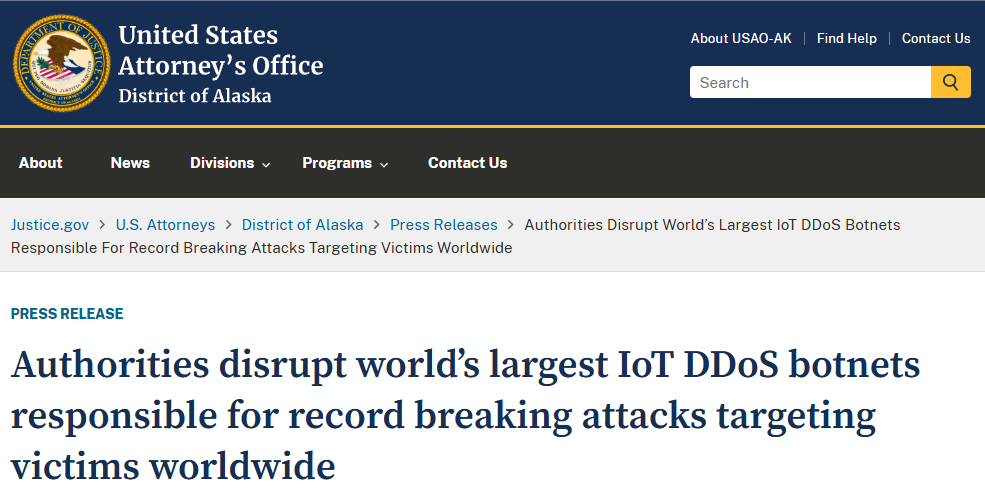
\includegraphics[width=0.8\textwidth]{Imagenes/05-bot.png} 
    \end{center} 

    % 4. Resumen y Análisis
    \section{Breve resumen de la noticia: (más de 100 palabras)}
    El Departamento de Justicia de los Estados Unidos, en una operación coordinada con fuerzas de seguridad de Canadá y Alemania, ha desmantelado la infraestructura de Comando y Control (C2) de cuatro de las botnets IoT más potentes del mundo. La intervención incluyó la ejecución de órdenes de incautación de dominios de internet registrados en EE. UU., servidores virtuales y otra infraestructura crítica utilizada para actividades criminales. Estas botnets habían esclavizado más de tres millones de dispositivos en todo el mundo, utilizándolos para ejecutar cientos de miles de ataques DDoS, algunos de los cuales establecieron récords de volumen de tráfico (30 Tbps). La operación no solo se limitó a la infraestructura técnica, sino que también incluyó acciones legales contra los individuos que operaban estas redes en el extranjero. Además de la interrupción técnica, se identificó que los criminales utilizaban estas redes para extorsionar a sus víctimas, exigiendo pagos para detener los ataques. La colaboración de gigantes tecnológicos como Amazon, Google y Cloudflare fue fundamental para identificar y mitigar la conectividad de estas redes ``zombie''.

    \section{Relación con la amenaza:}
    La noticia es un ejemplo paradigmático de la amenaza de las botnets, ilustrando cómo dispositivos domésticos e industriales vulnerables son reclutados de forma masiva para formar ejércitos digitales capaces de paralizar infraestructuras nacionales y servicios globales.

    \section{\textquestiondown Existe CVE o CWE asociado a la noticia?}
    La noticia no cita un CVE específico.

    \section{Impacto ocasionado por la amenaza en esta noticia: (más de 100 palabras)}
    El impacto documentado en esta operación es masivo, tanto a nivel técnico como económico. Financieramente, las víctimas han reportado pérdidas individuales de decenas de miles de dólares derivadas de los gastos de remediación y la interrupción de servicios. A nivel de infraestructura, el impacto es crítico: se lanzaron ataques que superaron los 30 Tbps, una cifra que puede saturar incluso las defensas más robustas de proveedores de servicios de internet y redes gubernamentales. La seguridad nacional también se vio comprometida, ya que las botnets dirigieron ataques específicamente contra la Red de Información del Departamento de Defensa (DoDIN). Además, el impacto social y de privacidad es notable, dado que más de tres millones de usuarios particulares poseían dispositivos (cámaras, routers) que estaban siendo utilizados para actividades delictivas sin su conocimiento. La escala de la infección subraya una vulnerabilidad sistémica en el ecosistema IoT global, donde la falta de seguridad en dispositivos de consumo se traduce en herramientas de ciberterrorismo y extorsión a gran escala.